\documentclass[tikz]{standalone}

\tikzstyle{node}=[draw=#1,fill=#1!20]

\newcommand{\vertex}[6]{\node[shape=circle,fill=black, scale=0.5,label=#1:{#2},label=#5:{\tiny\texttt{\color{blue}#6}},#4] (#3)  {};}
\newcommand{\myedge}[4]{ \draw[->] (#1) edge node[#2] {#3} (#4);}
\usetikzlibrary{automata}
\tikzset{
	initial text=\(\ast\),
}

\begin{document}
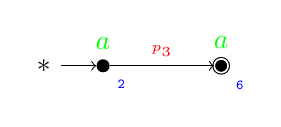
\begin{tikzpicture}[align=center,node distance=3cm]

        \vertex{above}{$\color{green}a$}{b}{initial}{below right}{2}
        \vertex{above}{$\color{green}a$}{b1}{right of=b,accepting,state,scale=0.4}{below right}{6}

    
   \draw[->] (b) edge node [above] {$\scriptscriptstyle{\color{red}p_3}$} (b1);
\end{tikzpicture}

\end{document}
